
\subsection{Scientific Context}
\label{sec:scientific context}

Data handling is becoming more and more important in environmental science, and consuming more and more of the computing budget.
This arises from the interplay of four key factors:
\begin{enumerate}
\item The direct influence of Moore's Law on instrumentation and simulation (finer resolution in space and time means more numbers),
\item The indirect influence of Moore's Law on what can be simulated (more compute means more things are computable),
\item The growth of interdisciplinarity (more things need to be compared and contrasted) and more people are doing it, and
\item The relationship between Moore's Law and Kryder's Law (is the cost of storage falling as rapidly as the cost of creating numbers to be storing is falling?).
\end{enumerate}

The influence of these four factors can be seen in several key climate data metrics: global archive estimates, CMIP archive sizes, institutional data growth, and the changing nature of science. (We concentrate here on climate science, since in terms of volume of data, climate science has a more existential problem than weather!)

\paragraph{Global Archives.}

In an attempt to quantify the data needed in global archives, Overpeck et al 2010 produced an estimate of data needed for globally available archives of data (reproduced here as \Cref{fig:data prediction climate}.
The provenance of the underlying data is unknown, but there are two general conclusions which can be drawn: (1) over the next decade global archive sizes will grow to o(hundreds of petabytes) in both of simulations and observations; and (2) it is likely that simulation growth will dominate over observation growth, particularly in the longer term.

\begin{figure}[h]
	\centering
	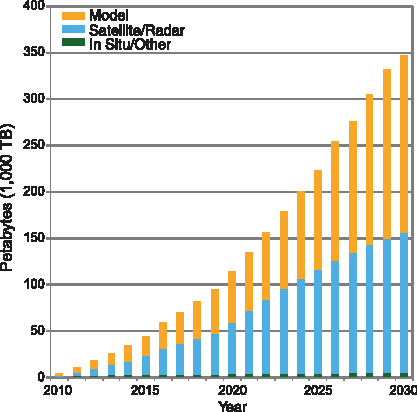
\includegraphics[width=0.5\linewidth]{3rd/overpeck_climate_2011-1_estimate-data-volume.pdf}
	\caption{Estimates of future archive volumes needed to support climate science \cite{overpeck_climate_2011}}
	\label{fig:data prediction climate}
\end{figure}

\paragraph{CMIP Archives.}

Globally coordinated Coupled Model Intercomparison Projects (CMIPs) are carried out at multi-year intervals, and involve many groups world wide running the same experiments and sharing data. With time the model resolutions increase, and so also do the number of experiments, the number of realisations of those experiments (the "ensemble size"), and the number of groups involved.

The influence of these factors can be seen in the direct comparison of data volumes produced for CMIP3 and CMIP5 shown in \Cref{tab:CMIP_data_volume}, and early estimates for CMIP6 (starting in 2017) varied between 30 and 300 PB.

The most recent UK assessments suggest the production of 3 PB of CMIP6 data within a joint modelling consortium. Given this group is likely to be attempting one of the largest ranges of CMIP6 experiments, and around 30 modelling groups, this latest data might suggest a maximum size for CMIP6 of 100 PB, but even so, it is likely that Overpeck's global projections for climate data are going to be significant under-estimates.

\begin{table}[htb]
	\small
	\centering
	\begin{tabular}{  l | c | r | r  }
		%\hline
		Centre & Country             &  CMIP3 (TB)& CMIP5 (TB) \\ \hline\hline
		BCC              & China               &  -                 & 51                \\
		BCCR             & Norway              & 0.862               & - \\
		CCCma            & Canada              & 2.071              & 51               \\
		CCSM, CESM       & USA                 & 9.173              & 739               \\
		CMCC             & Europe (Italy)      & -                  & 158            \\
		CNRM             & France              & 0.999               & 71              \\
		CSIRO            & Australia           & 2.088              & 81               \\
		EC-EARTH         & Europe (Netherland) &    -               & 97               \\
		GCESS            & China               &  -                 & 24               \\
		GFDL             & USA                 & 3.843              & - \\
		GISS             & USA                 & 1.097              & - \\
		IAP              & China               & 2.868              & - \\
		INGV             & Italy               & 1.472              & - \\
		INM              & Russia              & 0.366               & 30              \\
		IPSL             & France              & 0.998               & 121             \\
		LASG             & China               &  -                 & 100              \\
		MICRO/MICROC     & Japan               & 3.975              & 350              \\
		MIUB             & Germany/Korea       & 0.477               & - \\
		MOHC/UKMO            & UK                  &   0.973                & 195               \\
		MPI              & Germany             & 2.700              & 166              \\
		MRI              & Japan               & 1.025              & 269              \\
		NASA             & USA                 &  -                 & 375              \\
		NCC              & Norway              &   -                & 32               \\
		NCEP             & USA                 &   -                & 26                \\
		NIMR/KMA         & Korea               &   -                & 14               \\
		NOAA GFDL        & USA                 &   -                & 158              \\  \hline\hline
		Total            &                     & 34.989 (TB)       & 3,108 (TB)        \\
		%\hline          &
	\end{tabular}
	\caption{CMIP3 and CMIP5  Archive Volume (Credit: LLNL/Dean Williams)}
	\label{tab:CMIP_data_volume}
\end{table}

Looking forward beyond CMIP6, we note that the data intensity of climate model calculations is falling --- for the European contribution to CMIP5, the European Network for Earth Simulation (Andre et al, 2017, in preparation) reported an average ``production data intensity'' of 150 GB/1000 core-hours of compute, and estimate that for CMIP6 this is more like 30 GB/1000 core-hours. This falling intensity is in part because of the increase in model complexity, and in part because for many models an increase in resolution requires time-steps which are much shorter; both contribute to lower data intensity.  On the face of it, this might imply that as we move to exascale, we are likely to see even more dramatic decreases in data intensity, and while that is possible, we note that compute intensity remains the same if extra compute is spent on ensemble size. Unfortunately, this means it is hard to predict compute intensity far into the future based on these figures alone.

\paragraph{Local Archives.}
\label{sec:archive_intensity}

\begin{figure}
\centering
	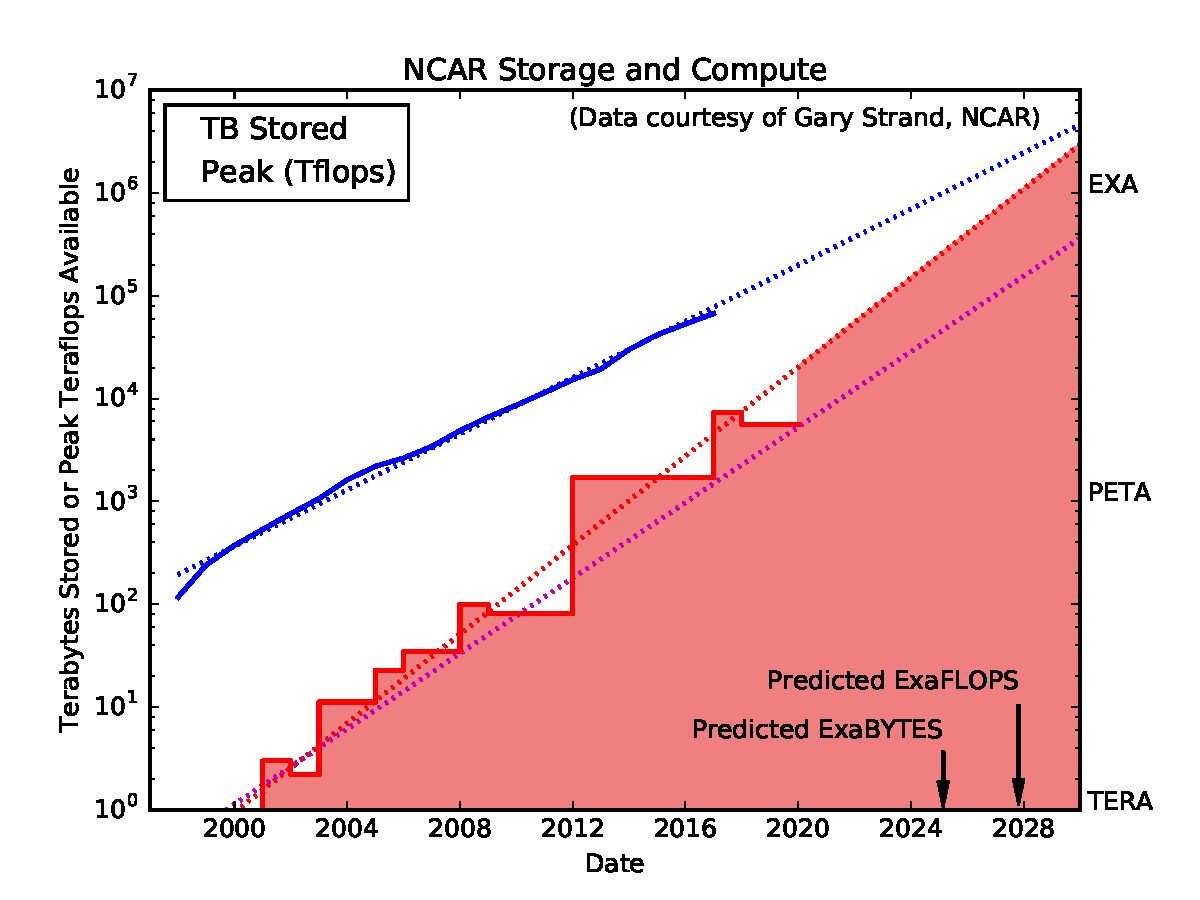
\includegraphics[width=0.7\linewidth]{figures/ncar_like_ncar.pdf}
	\caption{NCAR storage and compute. It is notable that NCAR expect to be handling an exabyte of data before they need to deal with exaflop computing.}
	\label{fig:ncar archive}\end{figure}

We are in the process of collecting local archive volume figures from key
weather and climate sites. One such site  is the US National Centre for Atmospheric Science (NCAR), who have a measurement of the total archive of data held at NCAR which can be correlated with the local compute (\Cref{fig:ncar archive}).  While the total archive includes both observation data and simulation data from other sites, it provides a useful measure of the change in data intensity, albeit via a proxy, which we here term the ``archive intensity''.  Simple back of the envelope calculations suggest that archive intensity will have gone from about 100 (TB/Tflop) in 2002 to about 10 in late 2027 when, if funding and technology were available, NCAR might be expecting to be dealing with 10 exabytes of data and an exascale compute resource.

Given that the archive intensity projection looks linear in log of the ratio, one could extrapolate the data intensity calculated for CMIP using the same assumption, which would lead to a prediction of production data intensity around 6-7 GB/1000 core hours in the mid-to-late 2020s, when we might expect it to be possible to be using exascale machines for climate science. However, on that timescale, the meaning of "cores" will have changed enough, that one might expect the data intensity in terms of core-hours used to have fallen even further.

\paragraph{Changing nature of science.}

The calculations thus far reflect the impact of extrapolation of ``business as usual''. One more important factor is the increasing scope of direct numerical simulation.  To assess how that is changing over time, we have examined\footnote{The assessment is very cursory, being based on the number of times certain phrases appear in Google Scholar citations, see \url{https://goo.gl/7q4v7H} for a complete description of the methodology.} the research literature for the use of terms which show the increasing impact of direct numerical simulation (and model inter-comparison projects) on current science. The data are shown in figure \ref{fig:citations}, and show that
\begin {enumerate}
\item  The number of papers on any facet of environmental science is growing (not unexpected, but used as a control).
\item The number of papers using direct numerical simulation is growing rapidly, but the use of DNS in environmental sciences is growing even more rapidly, at least using the proportional measure.
\item  The increase in papers which use MIP data is explosive, and one can see the direct influence of CMIP5 in the numbers.
\item Growth in observational science is slower than in numerical science, although the effect of increased availability of satellite data is apparent.
\end{enumerate}
The reason why these results are important in this context, is that they also demonstrate that data volumes are becoming an important issue for ever growing parts of the scientific community. Clearly the only way this can scale is that we replicate the data (expensive) or we improve the ability of data centres to support larger volumes and greater numbers of users!

\begin{figure}
\centering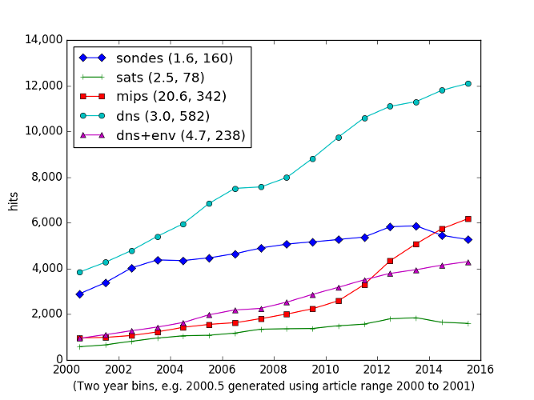
\includegraphics[width=0.7\linewidth]{3rd/google_searches.png}
\caption{The number of times certain phrases associated with direct numerical simulation (dns) or various aspects of observations (sondes, satellites) appear in the research literature. The numbers in the legend are firstly the ratio of the last couple of points over the first couple of points - a measure of proportional growth, and secondly, the gradient from a fit to the number of hits per annum - a measure of absolute growth.}
\label{fig:citations}
\end{figure}
